\documentclass[12pt]{article}

\usepackage[english]{babel}
\usepackage[utf8]{inputenc}
\usepackage{amsmath}
\usepackage{amsthm}
\usepackage{amsfonts}
\usepackage{fullpage}
\usepackage{subfiles}
\usepackage[hidelinks]{hyperref}
\usepackage{graphicx}
\usepackage{subfigure}
\usepackage{wrapfig}
\usepackage{tabularx}
\usepackage[ruled,vlined]{algorithm2e}
\usepackage{tikz}

% Command section 
\newcommand\numberthis{\addtocounter{equation}{1}\tag{\theequation}}
\newtheorem{theorem}{Theorem}[section]
\newtheorem{corollary}{Corollary}[theorem]
\newtheorem{proposition}{Proposition}[section]\newtheorem{definition}{Definition}[section]

% Allow page breaks in align environment
\allowdisplaybreaks

\begin{document}

\begin{titlepage}

    \newcommand{\HRule}{\rule{\linewidth}{0.5mm}} % Defines a new command for the horizontal lines, change thickness here



    \center % Center everything on the page

    %----------------------------------------------------------------------------------------
    %	HEADING SECTIONS
    %----------------------------------------------------------------------------------------

    \textsc{\LARGE Politecnico di Milano}\\[1.5cm] % Name of your university/college
    \textsc{\Large Machine Learning}\\[0.5cm] % Major heading such as course name
    \textsc{\large AA 2019/2020}\\[0.5cm] % Minor heading such as course title

    %----------------------------------------------------------------------------------------
    %	TITLE SECTION
    %----------------------------------------------------------------------------------------

    \HRule \\[0.4cm]
    { \huge \bfseries Summary - Machine Learning}\\[0.4cm] % Title of your document
    \HRule \\[1.5cm]

    %----------------------------------------------------------------------------------------
    %	AUTHOR SECTION
    %----------------------------------------------------------------------------------------

    %\begin{minipage}{0.4\textwidth}
    %\begin{flushleft}
    %\large \emph{Author:}\\
    %Valerio \textsc{Colombo}
    %\end{flushleft}
    %\end{minipage}
    %~
    %\begin{minipage}{0.4\textwidth}
    %\begin{flushright}
    %\large \emph{Professor:} \\
    %Marcello \textsc{Restelli} % Supervisor's Name
    %\end{flushright}

    %\end{minipage}\\[5cm]

    % If you don't want a supervisor, uncomment the two lines below and remove the section above
    \Large \emph{Author:}\\
    Valerio \textsc{Colombo}\\[3cm] % Your name

    %----------------------------------------------------------------------------------------
    %	LOGO SECTION
    %----------------------------------------------------------------------------------------

    
\includegraphics[scale=0.4]{images/Logo_Politecnico_Milano.png}\\[2cm] % Include a department/university logo - this will require the graphicx package

    %----------------------------------------------------------------------------------------
    %	COPYRIGHT SECTION
    %----------------------------------------------------------------------------------------

    \includegraphics[scale=0.4]{images/by-nc-sa.eps}\\[1cm]

    %----------------------------------------------------------------------------------------
    %	DATE SECTION
    %----------------------------------------------------------------------------------------

    {\large \today}\\[2cm] % Date, change the \today to a set date if you want to be precise

    %----------------------------------------------------------------------------------------

    \newpage

\end{titlepage}

\tableofcontents

\newpage

\subfile{sections/LinearRegression.tex}
\subfile{sections/LinearClassification.tex}
\subfile{sections/BiasVarianceTradeOff.tex}
\subfile{sections/PAC-Learning and VC-Dimension.tex}
\subfile{sections/KernelMethods.tex}
\subfile{sections/SupportVectorMachines.tex}
\subfile{sections/MDP.tex}
\subfile{sections/RLFinite.tex}
\subfile{sections/MAB.tex}

\end{document}
